% The cube of the U^3 norm (generated by a script).
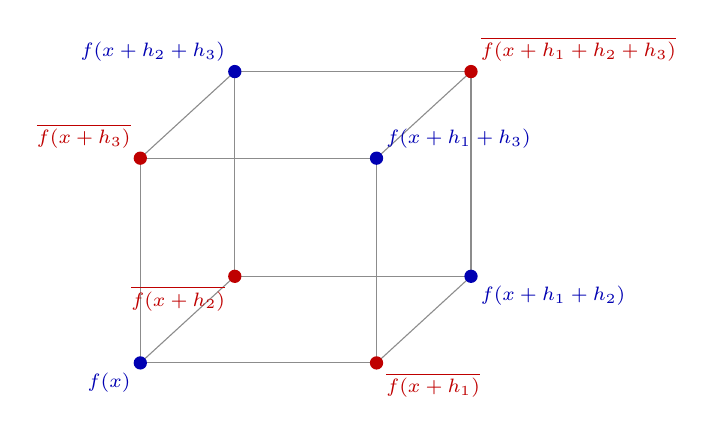
\begin{tikzpicture}[x=1cm,y=1cm]
\draw[black!45] (0.00,0.00)--(3.00,0.00);
\draw[black!45] (0.00,0.00)--(1.20,1.10);
\draw[black!45] (0.00,0.00)--(0.00,2.60);
\draw[black!45] (3.00,0.00)--(4.20,1.10);
\draw[black!45] (3.00,0.00)--(3.00,2.60);
\draw[black!45] (1.20,1.10)--(4.20,1.10);
\draw[black!45] (1.20,1.10)--(1.20,3.70);
\draw[black!45] (0.00,2.60)--(3.00,2.60);
\draw[black!45] (0.00,2.60)--(1.20,3.70);
\draw[black!45] (4.20,1.10)--(4.20,3.70);
\draw[black!45] (3.00,2.60)--(4.20,3.70);
\draw[black!45] (1.20,3.70)--(4.20,3.70);
\fill[blue!70!black] (0.00,0.00) circle (2.4pt);
\node[below left,font=\scriptsize,blue!70!black] at (0.00,0.00) {$f(x)$};
\fill[red!75!black] (3.00,0.00) circle (2.4pt);
\node[below right,font=\scriptsize,red!75!black] at (3.00,0.00) {$\overline{f(x+h_1)}$};
\fill[red!75!black] (1.20,1.10) circle (2.4pt);
\node[below left,font=\scriptsize,red!75!black] at (1.20,1.10) {$\overline{f(x+h_2)}$};
\fill[red!75!black] (0.00,2.60) circle (2.4pt);
\node[above left,font=\scriptsize,red!75!black] at (0.00,2.60) {$\overline{f(x+h_3)}$};
\fill[blue!70!black] (4.20,1.10) circle (2.4pt);
\node[below right,font=\scriptsize,blue!70!black] at (4.20,1.10) {$f(x+h_1+h_2)$};
\fill[blue!70!black] (3.00,2.60) circle (2.4pt);
\node[above right,font=\scriptsize,blue!70!black] at (3.00,2.60) {$f(x+h_1+h_3)$};
\fill[blue!70!black] (1.20,3.70) circle (2.4pt);
\node[above left,font=\scriptsize,blue!70!black] at (1.20,3.70) {$f(x+h_2+h_3)$};
\fill[red!75!black] (4.20,3.70) circle (2.4pt);
\node[above right,font=\scriptsize,red!75!black] at (4.20,3.70) {$\overline{f(x+h_1+h_2+h_3)}$};
\end{tikzpicture}
